\section*{8. Implementación y desarrollo}

\subsection{8.1 Implementación del backend con Django}

Durante la implementación del backend con Django, uno de los principales retos fue 
organizar la lógica de negocio de forma que el sistema fuese escalable, eficiente y 
capaz de integrar múltiples componentes como el scraping de datos, los modelos de 
Machine Learning, la caché y la comunicación en tiempo real.

\subsubsection{Modelado de datos}

El diseño de los modelos se planteó para representar de forma fiel el dominio del 
fútbol profesional y permitir tanto análisis estadístico como predicción. Para ello,
 se construyó una estructura relacional donde entidades como Jugador, Equipo, Partido
  y Jornada se interconectan mediante claves foráneas.

El núcleo del sistema es el modelo EstadisticasPartidoJugador, que almacena un 
conjunto muy amplio de variables (goles, asistencias, xG, duelos, métricas defensivas, 
etc.). Este modelo actúa como fuente principal de datos tanto para el análisis como
 para los modelos de Machine Learning.

Se incorporaron restricciones como \texttt{unique\_together} para garantizar la 
integridad (evitar duplicar estadísticas de un jugador en un mismo partido), 
así como validadores en múltiples campos. Además, se utilizaron campos JSON en varios modelos
 (roles, percentiles,etc.) para permitir mayor flexibilidad sin necesidad de 
 modificar el esquema constantemente.

Un aspecto especialmente relevante en el modelado de los datos fue la gestión de las posiciones
 de los jugadores. Las fuentes externas utilizadas durante el proceso de scraping presentan una 
 gran heterogeneidad en la nomenclatura de posiciones y roles (por ejemplo, ``MCF'' para mediocentro
  defensivo), lo que dificultaba su uso directo tanto en el análisis como en los modelos predictivos.

Para solucionar este problema, se optó por normalizar todas las posiciones en cuatro categorías 
principales: portero, defensa, centrocampista y delantero. Esta decisión simplifica el tratamiento 
de los datos y permite unificar criterios en todo el sistema.

Sin embargo, surgía un inconveniente adicional: muchos jugadores son polivalentes
y pueden desempeñar diferentes roles a lo largo de la temporada. Para abordar
esta situación, se implementó un método que calcula la posición más frecuente de
cada jugador en función de sus apariciones reales en partidos:

\begin{lstlisting}[language=Python,caption={Función para calcular posición más frecuente de un jugador}]
def get_posicion_mas_frecuente(self):
   posiciones = (
       self.estadisticas_partidos
       .filter(posicion__isnull=False)
       .values('posicion')
       .annotate(count=Count('id'))
       .order_by('-count')
       .first()
   )
 
   if posiciones:
       return posiciones['posicion']
   return None
\end{lstlisting}

Este enfoque permite asignar de forma dinámica una posición representativa basada en datos
 históricos, mitigando los problemas derivados de la polivalencia y mejorando la coherencia
  tanto en la visualización como en el entrenamiento de los modelos de Machine Learning.

\subsubsection{Implementación de la API}

La construcción de una API REST desde cero es una tarea compleja. Sin un framework especializado,
 habría que implementar manualmente:

\begin{itemize}
\item \textbf{Serialización:} Convertir objetos Python/ORM a JSON y validar datos entrantes.
\item \textbf{Autenticación y permisos:} Verificar quién es el usuario y qué puede hacer.
\item \textbf{Negociación de contenido:} Servir JSON, XML, etc. según lo que pida el cliente.
\item \textbf{Paginación:} Fragmentar resultados de 10.000 registros en bloques.
\item \textbf{Filtrado y búsqueda:} Aplicar criterios a consultas sin duplicar SQL.
\item \textbf{Estándares HTTP:} Retornar códigos de estado correctos (200, 400, 404, 500, etc).
\end{itemize}

Django REST Framework (DRF) abstrae toda esta complejidad mediante abstracciones de alto nivel
 que permiten construir APIs robustas en pocas líneas de código, siguiendo patrones estándar
  de la industria.

La API del proyecto se divide en dos versiones paralelas:

\begin{itemize}
\item \textbf{API v1:} Endpoints desarrollados incrementalmente durante las primeras fases del proyecto. Conviven endpoints dispares como \texttt{/api/predecir-portero/}, \texttt{/api/cambiar-jornada/}, \texttt{/api/plantilla/}, cada uno con su propia lógica de validación y respuesta. Aunque heterogénea, esta versión sigue activa porque ciertas funcionalidades depende de ella.

\item \textbf{API v2 (RESTful):} Una arquitectura más sistemática usando ViewSets de DRF, con endpoints jerárquicos como \texttt{/api/v2/jugadores/}, \texttt{/api/v2/equipos/}, \texttt{/api/v2/clasificacion/}. Sigue principios REST: operaciones CRUD sobre recursos claramente definidos, códigos HTTP semánticos, y paginación estándar.
\end{itemize}

Decisión de diseño: Mantener ambas en paralelo tiene un coste de mantenimiento,
 pero refleja más fielmente el proceso iterativo de desarrollo de un proyecto software.

\subsubsection{8.2.1 Serializers}

Un serializer en DRF es una clase que define cómo se transforma un objeto de Python
 (en este caso, un modelo Django) en una representación serializable (JSON) y 
 viceversa. Además de esta transformación, define explícitamente la estructura de
  los datos que se intercambian entre cliente y servidor, incluyendo sus tipos y 
  las reglas de validación que deben cumplirse. De este modo, el serializer actúa
   como el punto donde se formaliza el contrato de datos de la API.

A continuación se detalla la organización y funcionalidad algunos serializadores del proyecto:

\paragraph{Gestión de autenticación y validación de datos}

La seguridad y la integridad de los datos de usuario comienzan en el RegisterSerializer.
 A diferencia de un ModelSerializer estándar, esta clase permite un control total sobre el proceso de validación. 
 Implementa métodos específicos como \texttt{validate\_username} y \texttt{validate\_email} para garantizar la
  unicidad de las credenciales antes de la creación del registro. Además, el método \texttt{validate} actúa como 
  un filtro de seguridad final, verificando la coincidencia de contraseñas y aplicando las políticas de validación 
  nativas de Django.

\begin{lstlisting}[language=Python,caption={Validación de registro
con verificación de contraseñas en Django REST Framework}]
def validate(self, data):
    if data['password1'] != data['password2']:
        raise serializers.ValidationError({'password2': 'Las contrasenas no coinciden.'})
    try:
        validate_password(data['password1'])
    except Exception as e:
        raise serializers.ValidationError({'password1': list(e.messages)})
    return data
\end{lstlisting}

\paragraph{Perfiles de usuario y campos dinámicos}

Para ofrecer una respuesta rica en información sin múltiples consultas al servidor, el UserSerializer 
utiliza la capacidad de anidamiento de DRF para integrar el perfil extendido del usuario (UserProfile).
Un aspecto avanzado es el uso de SerializerMethodField, que permite generar atributos de solo lectura de
 forma programática. En este caso, se emplea para resolver la \texttt{foto\_url}, gestionando la 
lógica necesaria para extraer la ruta de la imagen del perfil o manejar 
excepciones si el recurso no existe.

\begin{lstlisting}[language=Python,caption={Serializer anidado con 
campos dinámicos usando SerializerMethodField}]
class UserSerializer(serializers.ModelSerializer):
    profile = UserProfileSerializer(read_only=True)
    foto_url = serializers.SerializerMethodField()

    def get_foto_url(self, obj):
        try:
            if obj.profile.foto:
                return obj.profile.foto.url
        except Exception:
            pass
        return None
\end{lstlisting}

\paragraph{Relaciones sociales}

La gestión de amistades requiere una lógica que identifique correctamente a los participantes de la relación
 según quién realice la consulta. El AmistadSerializer resuelve esta ambigüedad accediendo al contexto de la 
 petición para determinar cuál de los dos usuarios en el modelo Amistad es el ``amigo'' del usuario
  autenticado. Por otro lado, serializadores como SolicitudAmistadSerializer utilizan el parámetro \texttt{source}
   para crear alias legibles (como \texttt{emisor\_username}) a partir de relaciones de clave foránea, simplificando
 la estructura del JSON para el frontend.

\begin{lstlisting}[language=Python,caption={Resolución ambigua de 
relaciones sociales en serializers mediante context}]
def _amigo(self, obj):
    req = self.context.get('request')
    return obj.usuario2 if obj.usuario1 == req.user else obj.usuario1

def get_amigo_username(self, obj): 
    return self._amigo(obj).username
\end{lstlisting}

\paragraph{Serialización de recursos genéricos}

Finalmente, el módulo incluye serializadores de solo lectura para recursos básicos como Equipos
, Jugadores y Plantillas. Estos están diseñados para ser eficientes en operaciones de listado masivo,
 devolviendo únicamente los campos esenciales requeridos por la interfaz, como el nombre, la nacionalidad
  o la formación táctica, garantizando un rendimiento óptimo de la API al minimizar la carga de datos transferidos.

\subsubsection{8.1.2 Implementación de la lógica de negocio}

La arquitectura del backend se ha diseñado siguiendo un principio de modularidad estricta y desacoplamiento.
 Para gestionar la alta complejidad de las reglas de negocio deportivo y la integración de modelos predictivos, 
 el directorio \texttt{api/} se fragmentó en módulos especializados. Esta estructura no solo facilita el mantenimiento preventivo,
  sino que permite optimizar de forma aislada componentes críticos como la inferencia de Machine Learning, la búsqueda avanzada o el procesamiento estadístico masivo.

A continuación, se detallan las soluciones técnicas implementadas, agrupadas por su funcionalidad dentro del ecosistema de la aplicación:
\begin{figure}[H]
\centering
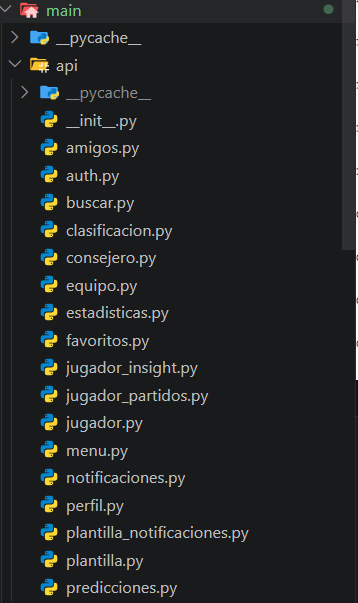
\includegraphics[width=0.3\textwidth]{./images/api.png}
\caption{Captura real de la organización del módulo de api/.}
\end{figure}




\subsubsection{8.1.2.1 Gestión de identidad y entorno social}

Este bloque gestiona el ciclo de vida del usuario y su interacción social. \texttt{auth.py} centraliza la identidad
 asegurando la integridad mediante un helper centralizado (\texttt{\_user\_info}) que inyecta datos del perfil y resuelve
  la seguridad CSRF. \texttt{perfil.py} extiende esto con la lógica de privacidad y la gestión de aquellos sucesos que lanzan una notificación. 

La capa social reside en \texttt{amigos.py}, que implementa un sistema reactivo de solicitudes que dispara avisos mediante \texttt{notificaciones.py}. 
Para personalizar la experiencia, \texttt{favoritos.py} persiste las preferencias de clubes, permitiendo que el resto de la API filtre ránkings y calendarios de forma automática.

\subsubsection{8.1.2.2 Motor de búsqueda, clasificación y agregación de estadísticas}

Este bloque constituye el núcleo analítico del sistema, encargándose de transformar volúmenes masivos de métricas en bruto en información estructurada,
 ránkings comparativos y narrativas de partido. El módulo \texttt{buscar.py} actúa como la interfaz de abstracción sobre el motor MeiliSearch, implementando
  búsquedas de texto con lógica difusa sobre jugadores y equipos, aplicando pesos dinámicos para priorizar coincidencias exactas. Complementando esta 
  capa, \texttt{jugador\_insight.py} utiliza un motor heurístico que pondera estadísticas clave según la demarcación del futbolista para generar conclusiones
   semánticas dinámicas, transformando datos numéricos en información de valor deportivo.

Por su parte, \texttt{estadisticas.py} implementa un motor de búsqueda global con filtrado avanzado por jornadas. Su mayor valor técnico reside en el 
tratamiento de la integridad de datos mediante la detección de outliers: el sistema identifica puntuaciones anómalas superiores a 40 puntos (frecuentes por errores en fuentes externas)
 y las sustituye por la moda estadística del jugador para no sesgar las medias. Asimismo, resuelve el reto de la comparativa justa mediante el cálculo dinámico de percentiles relativos
  por posición, permitiendo determinar el rango real de un jugador dentro de su rol específico.

\begin{lstlisting}[language=Python,caption={Cálculo dinámico de 
percentiles relativos por posición}]
for pos, jugadores_pos in jugadores_por_posicion.items():
    for stat_key in stats_to_calc:
        values = [r.get(stat_key, 0) for r in jugadores_pos]
        if values and len(values) > 1:
            for row in jugadores_pos:
                val = row.get(stat_key, 0)
                count_lower = sum(1 for v in values if v < val)
                count_equal = sum(1 for v in values if v == val)
                percentil = int(((count_lower + count_equal * 0.5) / len(values)) * 100)
                row[f'{stat_key}_percentil'] = max(0, min(100, percentil))
\end{lstlisting}

Finalmente, \texttt{clasificacion.py} se encarga de reconstruir la tabla de posiciones dinámicamente para cualquier jornada de la temporada. Su funcionalidad más
 compleja es el método \texttt{\_build\_sucesos}, que realiza un cruce relacional entre las estadísticas de cada jugador y los eventos del partido para generar
  una cronología narrativa. Este proceso transforma datos tabulares en una lista estructurada de sucesos (goles, tarjetas y asistencias) asignados dinámicamente 
  al contenedor local o visitante, permitiendo que el frontend renderice una lista cronológica de lo ocurrido en 
cada encuentro de la jornada seleccionada.

\begin{lstlisting}[language=Python,caption={Reconstrucción de 
eventos del partido mediante cruce relacional}]
def _build_sucesos(partido_jugado, temporada):
    sucesos = {'goles_local': [], 'goles_visitante': [], 'amarillas_local': [], ...}
    for stats in EstadisticasPartidoJugador.objects.filter(partido=partido_jugado).select_related('jugador'):
        ejt = EquipoJugadorTemporada.objects.filter(jugador=stats.jugador, temporada=temporada).first()
        if not ejt: continue
        
        target = 'local' if ejt.equipo == partido_jugado.equipo_local else 'visitante'
        nombre = f"{stats.jugador.nombre} {stats.jugador.apellido}".strip()
        
        if stats.gol_partido > 0:
            for _ in range(stats.gol_partido):
                sucesos[f'goles_{target}'].append({'nombre': nombre, 'minuto': stats.min_partido})
        
        if stats.amarillas > 0:
            sucesos[f'amarillas_{target}'].append({'nombre': nombre, 'minuto': stats.min_partido})
            
    return sucesos
\end{lstlisting}

\subsubsection{8.1.2.3 Detalles de los equipos}

El archivo \texttt{equipo.py} actúa como un motor de análisis comparativo. Para evitar el problema de rendimiento N+1, se implementó una precomputación
 de consultas (\texttt{annotate} y \texttt{Count}) que recupera la lista de jugadores por temporada en una única llamada. La vista \texttt{EquipoDetailView} construye 
 un objeto \texttt{rival\_info} 
dinámico que permite comparar racha y H2H (Head-to-Head) en tiempo real.

\begin{lstlisting}[language=Python,caption={Construcción de objeto 
de análisis comparativo entre equipos rivales}]
rival_info = {
    'nombre': rival.nombre,
    'escudo': shield_name(rival.nombre),
    'racha': racha_rival_detalles,
    'goles_favor': goles_rival_favor,
    'h2h': get_h2h_historico(equipo, rival, temporada),
    'max_goleador_rival': max_goleador_rival,
    'partido_anterior': partido_anterior,
}
\end{lstlisting}

Además, el sistema muestra un top 3 dinámico según la jornada y ciertas 
estadísticas significativas:

\begin{lstlisting}[language=Python,caption={Generación de ranking top 3}]
jugadores = sorted(jugadores_agrupados.values(), key=lambda x: x['total_puntos'], reverse=True)
top_3_puntos = jugadores[:3] # Lideres en puntos
top_3_minutos = sorted(jugadores, key=lambda x: x['total_minutos'], reverse=True)[:3] # Lideres en participacion
\end{lstlisting}

\subsubsection{8.1.2.4 Perfil del jugador}

\texttt{jugador.py} gestiona el perfil detallado y el histórico de carrera (\texttt{jugador\_partidos.py}). El mayor reto aquí es la integridad de
 los datos; los cálculos de percentiles y xG generan a menudo valores compatibles con la lógica matemática pero incompatibles con JSON (NaN o Inf).
  Se desarrolló el \texttt{NaNInfEncoder}, un codificador personalizado que 
sanitiza la salida para evitar errores de parsing en el cliente cuando aparecen estos valores críticos.

\begin{lstlisting}[language=Python,caption={Codificador JSON personalizado}]
class NaNInfEncoder(json.JSONEncoder):
    def iterencode(self, o, _one_shot=False):
        for chunk in super().iterencode(o, _one_shot):
            # Limpieza proactiva para evitar fallos de parsing en el frontend
            chunk = chunk.replace('NaN', '0').replace('Infinity', '0').replace('-Infinity', '0')
            yield chunk
\end{lstlisting}

\subsubsection{8.1.2.5 Generación y explicación de predicciones}

\texttt{predicciones.py} y \texttt{consejero.py} forman el núcleo de IA. El orquestador de ML implementa una estrategia de predicción híbrida: durante 
las primeras 5 jornadas (muestra insuficiente) activa un fallback de 
``Media Histórica''; a partir de la 6, conmuta a inferencia pura de ML, 
devolviendo márgenes de error y rangos de confianza.

\begin{lstlisting}[language=Python,caption={Estrategia de predicción híbrida}]
if jornada_num <= 5:
    media_puntos = jugador.estadisticas_partidos.aggregate(media=Avg('puntos_fantasy'))['media']
    return Response({'status': 'success', 'prediccion': round(float(media_puntos), 2), 'modelo': 'Media Historica'})
else:
    resultado = predecir_puntos_portero(nombre_jugador, jornada, modelo_tipo=modelo_tipo)
    return Response({'prediccion': float(resultado['prediccion']), 'margen': float(resultado.get('margen', 0))})
\end{lstlisting}

Se añade además una capa de IA Explicable (XAI) mediante SHAP, permitiendo que el sistema justifique cada decisión basándose y exponiendo los factores de mayor impacto.

\subsubsection{8.1.2.6 Gestión de alineaciones}

Este pack gestiona la lógica de juego y el seguimiento en tiempo real.  \texttt{plantilla.py} actúa como el motor de construcción de alineaciones, 
validando formaciones (ej. 4-3-3, 4-4-2, etc.) y calculando puntos en tiempo real. Se apoya en \texttt{plantilla\_notificaciones.py}, un monitor reactivo 
que detecta eventos en vivo (goles, tarjetas o asistencias) de los jugadores alineados por el usuario.

\begin{lstlisting}[language=Python,caption={Detección de eventos en 
vivo con sistema de claves únicas para evitar redundancias}]
for stat in stats:
    if stat.gol_partido > 0:
        key = f"{stat.jugador_id}_gol"
        if key not in seen:
            eventos.append({'jugador_id': stat.jugador_id, 'evento': 'gol', 'equipo': _get_equipo(stat)})
            seen.add(key)
\end{lstlisting}

Finalmente, como medida aviso, la API rastrea la participación 
reciente e inyecta alertas si un jugador suma menos de 60 minutos en los 
últimos 4 partidos, protegiendo al usuario ante posibles suplencias:

\begin{lstlisting}[language=Python,caption={Sistema de alertas 
para jugadores con bajo minutaje}]
pocos_minutos_set = {
    jid for jid, mins in _min_sum.items()
    if mins and sum(mins) < 60
}
'pocos_minutos': jugador.id in pocos_minutos_set,
\end{lstlisting}

\subsubsection{8.1.2.7 Orquestación}

Dado que el cálculo de percentiles y rankings estadísticos requiere procesar miles de registros de EstadisticasPartidoJugador,
 el coste computacional es elevado. Para mantener tiempos de respuesta óptimos, se implementó un sistema de caché utilizando
 el backend de caché de Redis.
 
Las funciones que generan rankings y agregaciones almacenan los resultados en caché mediante claves únicas asociadas a la 
temporada y jornada, usando cache.set. Esto permite servir respuestas instantáneas para consultas repetidas, y el contenido se 
invalida automáticamente tras un periodo de expiración o cuando se detectan cambios en los datos relevantes.

\subsubsection{8.1.3 Arquitectura reactiva y optimización de rendimiento}

Tras implementar la lógica de los endpoints, se desarrollaron una serie de componentes transversales encargados de automatizar tareas, asegurar 
la comunicación bidireccional y garantizar la fluidez de la plataforma bajo carga de datos masiva.

\subsubsection{8.1.3.1 Automatización mediante Signals}

Para mantener el desacoplamiento del código, se utilizó el patrón Observer mediante los Django Signals. Esto permite que el sistema reaccione a 
eventos en la base de datos sin necesidad de ensuciar las vistas con lógica adicional. Se implementaron tres flujos críticos:

\begin{itemize}
\item Indexación en MeiliSearch: cada vez que un Jugador o Equipo es creado o actualizado, una señal \texttt{post\_save} actualiza automáticamente el índice en el motor de búsqueda, garantizando que los resultados de búsqueda estén siempre sincronizados.
\item Auto-predicción en segundo plano: al recibir nuevas estadísticas de un partido, el sistema dispara automáticamente el cálculo de la predicción para la siguiente jornada.
\item Gestión de perfiles: creación automática de la entidad UserProfile al registrar un nuevo usuario en el sistema auth.
\end{itemize}

\subsubsection{8.1.3.2 Comunicación en tiempo real con WebSockets}

Para las notificaciones (goles en directo, solicitudes de amistad), una API REST convencional obligaría al cliente a realizar polling constante,
 saturando el servidor. Para solventarlo, se implementó una capa de WebSockets utilizando Django Channels.

Se desarrolló el \texttt{NotificacionConsumer}, un componente asíncrono que 
mantiene una conexión persistente con cada cliente autenticado. Cuando una 
señal detecta un evento relevante, este se envía al grupo de canales del 
usuario afectado, permitiendo una experiencia de usuario totalmente reactiva.

\begin{lstlisting}[language=Python,caption={Signal de Django para 
emitir notificaciones en tiempo real vía WebSockets}]
@receiver(post_save, sender=Notificacion)
def notificacion_creada_ws(sender, instance, created, **kwargs):
    if created:
        channel_layer = get_channel_layer()
        async_to_sync(channel_layer.group_send)(
            f'notificaciones_{instance.usuario_id}',
            {
                'type': 'notificacion_nueva',
                'notificacion': serialize_notif(instance)
            }
        )
\end{lstlisting}

\subsubsection{8.1.3.3 Estrategia de caching y optimización de agregaciones}

Dado que el cálculo de percentiles y ránkings estadísticos requiere procesar miles de registros de \texttt{EstadisticasPartidoJugador}, el
 coste computacional es elevado. Para mantener tiempos de respuesta que no afecten a la experiencia de usuario, se diseñó un sistema de caché basado en Redis.

Se implementó un decorador personalizado, \texttt{@cache\_api\_response}, que genera una clave única basada en la URL y los parámetros de la consulta. 
Esto permite servir datos idénticos de forma instantánea, invalidando el contenido automáticamente según el ciclo de actualización de las jornadas.

\subsubsection{8.1.4 Arranque y ciclo de vida}

Para garantizar la robustez del sistema desde el momento del despliegue, se ha implementado una lógica de inicialización avanzada en el 
componente \texttt{apps.py}. Este módulo no solo registra la configuración de la aplicación, sino que actúa como un orquestador de integridad, 
asegurando que todos los servicios dependientes (Base de Datos, MeiliSearch y Modelos de ML) estén sincronizados y listos para operar.

\subsubsection{8.1.4.1 Inicialización asíncrona y gestión de cold start}

Uno de los retos técnicos resueltos fue evitar el bloqueo del servidor durante el arranque. Si el sistema realizara comprobaciones pesadas de
 datos en el hilo principal, el servidor web podría interrumpir el proceso por timeout.

Para solventarlo, se implementó un sistema de inicialización en segundo plano 
mediante \texttt{threading.Thread}. Al arrancar Django, el método \texttt{ready()} 
dispara un hilo que ejecuta un pipeline de 5 pasos  
sin impedir que el servidor comience a escuchar peticiones.

\begin{lstlisting}[language=Python,caption={Inicialización 
asíncrona en hilo durante startup de Django}]
def ready(self):
    if 'runserver' in sys.argv:
        init_thread = threading.Thread(target=self._initialize_data, daemon=True)
        init_thread.start()
\end{lstlisting}

\subsubsection{8.1.4.2 Pipeline de arranque}

La función \texttt{\_initialize\_data} ejecuta la lógica de iniciar el servidor, dividida en cinco fases:

\begin{enumerate}
\item Auditoría de persistencia: comprueba el volumen de registros en Partido y Estadisticas. Si detecta una base de datos vacía, marca el sistema como ``incompleto''.
\item Carga masiva de datos: si la comprobación falla, invoca el módulo de scraping para poblar la base de datos desde cero. Un detalle técnico relevante es la desconexión temporal de Signals durante esta fase; esto evita que se disparen miles de hilos de predicción innecesarios durante una carga masiva, optimizando el uso de CPU y memoria.
\item Verificación de roles: asegura que los campos JSON de roles (corners, penaltis) estén poblados, lanzando procesos de limpieza si detecta una carencia superior al 50\%.
\item Sincronización con el motor de búsqueda: verifica la disponibilidad del cliente MeiliSearch y fuerza una reindexación completa de jugadores y equipos.
\item Pre-generación de inferencias: identifica jornadas de la temporada actual sin predicciones y lanza el comando de generación para que el usuario disponga de datos predictivos desde el primer minuto.
\end{enumerate}

\subsubsection{8.1.4.3 Pre-carga de módulos de Machine Learning}

Para optimizar el rendimiento de la primera petición (latencia de ``primer acceso''), se ha incluido una lógica de pre-importación del módulo \texttt{predecir.py}. 
Esto asegura que el grafo de computación y las librerías pesadas (como Scikit-Learn o XGBoost) ya estén en la memoria RAM del proceso worker antes de que llegue la 
primera consulta del usuario, reduciendo el tiempo de respuesta inicial de varios segundos a milisegundos.

\subsection{8.2 Implementación del scraping de datos}

La construcción del dataset maestro ha sido uno de los retos de ingeniería más exigentes del proyecto. A diferencia de otros dominios donde existen APIs públicas,
 el ecosistema del fútbol requiere la extracción de datos desde múltiples fuentes web heterogéneas. La implementación se ha estructurado en scripts especializados 
 que gestionan la descarga, el bypass de protecciones y el parseo de estructuras HTML complejas, garantizando la integridad de más de 23.000 registros históricos.

\subsubsection{8.2.1 Origen de los datos y fuentes}

Se han integrado tres fuentes principales para cubrir todas las dimensiones del sistema:

\begin{itemize}
\item \textbf{FBRef:} fuente principal de métricas avanzadas (xG, PSxG, progresiones, estadísticas defensivas y de portería).
\item \textbf{FutbolFantasy:} utilizada exclusivamente para la obtención de  los puntos obtenidos por cada jugador en la plataforma oficial.
\item \textbf{Transfermarkt:} fuente de contexto competitivo, empleada para extraer las rachas de los equipos, datos de estadios, calendario y nacionalidades.
\end{itemize}

\subsubsection{8.2.2 Gestión de barreras técnicas y bloqueos}

Durante el desarrollo, se detectaron barreras críticas de seguridad que obligaron a diseñar estrategias de mitigación específicas:

\begin{itemize}
\item Bloqueos de IP en FBRef: este portal implementa políticas extremadamente estrictas de rate limiting. Ante la imposibilidad de realizar un scraping masivo 
automatizado sin ser baneado, se tomó una decisión de diseño basada en la gestión de riesgos: la descarga controlada y local de los archivos HTML. Se procesaron 
de forma secuencial los HTML de los partidos de las últimas tres temporadas (23/24, 24/25 y la actual 25/26), asegurando la persistencia de los datos sin comprometer 
la disponibilidad del sistema.

\item Evasión de Cloudflare en FutbolFantasy: el sitio bloquea agentes no humanos. Se implementó el módulo \texttt{descargar\_puntos.py} utilizando la librería \texttt{cloudscraper}, que permite simular una huella de navegador real, gestionando automáticamente los desafíos de JavaScript y cabeceras User-Agent.
\end{itemize}

\subsubsection{8.2.3 Algoritmo de reintentos}

Para garantizar la robustez de las descargas en FutbolFantasy, se desarrolló 
un algoritmo con reintentos y esperas aleatorias. Esto evita que el servidor 
identifique patrones de automatización y permite recuperarse de errores 
temporales de red.

\begin{lstlisting}[language=Python,caption={Algoritmo de 
reintentos para descargas robustas}]
def descargar_html_con_reintentos(url, max_intentos=5):
    intento = 0
    while intento < max_intentos:
        intento += 1
        try:
            resp = scraper.get(url, timeout=30)
            if resp.status_code == 200:
                return resp.text
        except Exception as e:
            delay = min(3.0 * (2 ** (intento - 1)), 30.0) + random.uniform(0, 1.5)
            time.sleep(delay)
    raise RuntimeError(f"Fallo tras {max_intentos} intentos en {url}")
\end{lstlisting}

\subsubsection{8.2.4 Módulos técnicos y responsabilidades}

La lógica de scraping se divide en archivos especializados para maximizar la mantenibilidad del pipeline:

\paragraph{A. descargar\_puntos.py}

Este módulo representa el punto de entrada del pipeline, encargado de la descarga masiva de documentos HTML. Su arquitectura contempla la evasión
 de sistemas de seguridad perimetral comunes en portales de alta demanda.

\begin{itemize}
\item Gestión de sesiones: implementa la librería \texttt{cloudscraper} para mitigar los bloqueos por desafíos de JavaScript de Cloudflare, simulando un entorno de navegación real (User-Agent dinámico, cabeceras de conexión persistente).

\item Estrategia de reintentos: utiliza un algoritmo de backoff exponencial con varianza aleatoria. Esto evita la saturación del servidor y reduce la detección de patrones de tráfico automatizado.

\item Comprobaciones: el sistema verifica la integridad y existencia de archivos locales antes de iniciar la descarga.
\end{itemize}

\begin{lstlisting}[language=Python,caption={Reintento con espera aleatoria para mitigación de detección de bots}]
delay_base = min(backoff_inicial * (2 ** (intento - 1)), backoff_max)
delay = delay_base + random.uniform(0, 1.5)
time.sleep(delay)
\end{lstlisting}

Nota de implementación: debido a las políticas de seguridad extremadamente restrictivas detectadas durante la fase de ejecución (bloqueos por IP tras descargas masivas),
 este script sirvió como base de pruebas, aunque la obtención del grueso de los datos históricos se complementó con descargas manuales controladas para asegurar la integridad
  de la base de datos.

\paragraph{B. commons.py}

Es el motor de procesamiento de texto que garantiza la cohesión entre diferentes fuentes de datos.

\begin{itemize}
\item Limpieza de cadenas: implementa expresiones regulares para eliminar información residual en los nombres de los jugadores (como los minutos jugados que FBRef concatena al nombre en ciertos nodos, ej: 90+4').

\item Normalización: utiliza la normalización NFD (Normalization Form Decomposition) para separar caracteres base de sus acentos, eliminando sistemáticamente los diacríticos. Esto es vital para asegurar que ``Martínez'' y ``Martinez'' sean tratados como el mismo registro.
\end{itemize}

\paragraph{C. fbref.py}

Este es el script más complejo a nivel de lógica de negocio, ya que debe unificar múltiples dimensiones estadísticas de un mismo encuentro y enriquecer 
los datos con atributos derivados. Su arquitectura está centrada en la integración de datos heterogéneos y la verificación de integridad por partido.

\begin{itemize}
\item Procesado de tablas: FBRef estructura los datos por encuentro en múltiples tablas HTML con identificadores específicos (tabla ID contiene ``\_home\_'' o ``\_away\_'' según del equipo). La función \texttt{parsear\_tabla\_fbref()} emplea BeautifulSoup para localizar tables dinámicamente, normalizar nombres de columnas y combinar filas de múltiples tablas usando el nombre normalizado del jugador como clave de unión (inner join en memoria).

\item Manejo especializado para porteros: dado que los porteros comparten tablas parcialmente distintas con métricas específicas (PSxG, Save\%, GA90), la función \texttt{buscar\_estadisticas\_portero()} implementa una estrategia jerárquica: búsqueda por nombre exacto $\rightarrow$ búsqueda por apellido. Esto garantiza que el 100\% de porteros sean asociados correctamente incluso cuando existen inconsistencias menores en los datos de FBRef.

\item Extracción de calendario: además de las métricas, parsea los resultados históricos y las fechas de los encuentros para construir la base del calendario de la competición.
\end{itemize}

\paragraph{D. transfermarkt.py}

Mientras FBRef aporta datos intrínsecos del jugador, este módulo recupera variables extrínsecas mediante \texttt{parse\_tabla\_jornada\_transfermarkt()}, extrayendo de forma confiable:

\begin{itemize}
\item Posición en clasificación (PJ, PG, PE, PP, puntos)
\item Diferencia de goles (GF, GC, DF, etc.)
\end{itemize}

\paragraph{E. roles.py}

Módulo avanzado diseñado para detectar jugadores que destacan especialmente en categorías estadísticas específicas(córners, asistencias, etc.).

\begin{itemize}
\item Parseo de elementos ocultos: los datos de rankings en FBRef se cargan de forma asíncrona o se encuentran dentro de comentario HTML . \texttt{roles.py} implementa una técnica de extracción de comentarios mediante BeautifulSoup para acceder a esta información.

\item Mapeo semántico: transforma ránkings numéricos en descripciones 
narrativas (insights), permitiendo que el sistema genere automáticamente 
conclusiones para la interfaz de usuario.
\end{itemize}

\begin{lstlisting}[language=Python,caption={Extracción de nodos 
comentario HTML con BeautifulSoup para datos ocultos}]
comments = soup.find_all(string=lambda text: isinstance(text, Comment))
for c in comments:
    if 'id="div_leaders"' in c:
        frag_soup = BeautifulSoup(c, "lxml")
\end{lstlisting}

\subsubsection{8.2.5 Identificación de roles}

Este proceso es vital para el enriquecimiento del dataset. El sistema localiza a los jugadores que ocupan el top 10 en ránkings de eficiencia 
(goles por disparo, pases al último tercio, intercepciones, etc.). Estos datos permiten al modelo de predicción asignar un peso mayor a jugadores 
que, independientemente de sus puntos brutos, demuestran una importancia táctica superior en la liga.

Los roles se almacenan en un objeto JSON donde la clave principal es el nombre normalizado del jugador, facilitando un acceso rápido durante el entrenamiento.
 Cada registro contiene una lista de los ránkings donde el jugador es protagonista, almacenando la posición y el valor absoluto de la métrica.

Ejemplo de formato JSON generado:

\begin{lstlisting}[language=Python,caption={Estructura JSON de roles y rankings de eficiencia para enriquecimiento de features}]
{
  "lamine yamal": [
    {"regates_exitosos": [1, 45.2]},
    {"pases_clave": [3, 12]},
    {"asistencias": [2, 7]}
  ],
  "antonio rudiger": [
    {"despejes": [5, 88]},
    {"intercepciones": [10, 32]}
  ]
}
\end{lstlisting}

\subsubsection{8.2.6 Orquestación del scraping}

El paso final de scraping es el script \texttt{popularDB.py}, que representa la fase de consolidación de datos. Este script ejecuta secuencialmente:

\begin{enumerate}
\item Validación de disponibilidad local: comprueba la existencia de los HTML de FBRef descargados previamente, evitando depender de peticiones masivas en tiempo real y reduciendo el riesgo de bloqueos por IP.
\item Carga de entidades base: crea en la base de datos las temporadas, equipos y jornadas necesarias para estructurar el resto de la información.
\item Ensamblaje de estadísticas por partido y jugador: integra los datos procedentes de fbref.py, transfermarkt.py y roles.py en registros unificados con múltiples atributos por jugador-partido.
\item Normalización de datos: aplica las reglas de homogeneización definidas en el sistema para asegurar consistencia entre fuentes antes de la persistencia.
\item Agregación histórica: genera el rendimiento histórico del jugador a partir de sus estadísticas acumuladas en la temporada.
\item Persistencia final: guarda los datos intermedios en CSV y los consolida en PostgreSQL, cerrando así la fase de ingestión.
\end{enumerate}

Esta orquestación permite desacoplar la extracción de datos de su consolidación, facilitando la trazabilidad, la recuperación ante errores y 
la reutilización de los distintos módulos del pipeline.

\subsection{8.3 Implementación del matching de entidades}

El primer paso es reducir el ``ruido'' textual. Antes de cualquier comparación, el sistema aplica una normalización agresiva:

\begin{itemize}
\item Conversión a minúsculas y eliminación de tildes.
\item Eliminación de caracteres especiales (guiones, puntos).
\item Limpieza de minutos: FBRef a veces incluye el minuto del evento en el nombre del jugador en el HTML; el sistema lo detecta y limpia mediante expresiones regulares a través del módulo \texttt{commons.py}.
\end{itemize}

\begin{lstlisting}[language=Python,caption={Normalización de texto y limpieza de minutos para entity matching}]
def normalizar_texto(texto):
    texto = str(texto).lower().strip()
    texto = unicodedata.normalize("NFD", texto)
    texto = "".join(c for c in texto if unicodedata.category(c) != "Mn")
    texto = re.sub(r"[-.]", " ", texto)
    texto = re.sub(r"\s+", " ", texto)
    return texto.strip()

def limpiar_minuto(nombre: str) -> str:
    if not nombre: return nombre
    nombre = nombre.replace("+", "").replace("-", "").strip()
    nombre = re.sub(r"\s*\d+(?:\+\d+)?'?$", "", nombre).strip()
    return nombre
\end{lstlisting}

\subsubsection{8.3.1 Alias por temporada y casos especiales}

Existen casos donde la normalización no es suficiente (ej. ``Pepelu'' no se parece a ``José Luis García Vaya''). El sistema utiliza un diccionario 
de alias que mapea nombres conocidos según la temporada y el equipo. Esto permite interceptar estos casos antes de que lleguen a la lógica probabilística.

Ejemplos de flujo:

\begin{itemize}
\item (Alias) Isaac Palazón Camacho $\rightarrow$ Isi (Rayo Vallecano)
\item (Normalización) Alexander Sørloth $\rightarrow$ Sorloth (Villarreal/Atlético)
\end{itemize}

\subsubsection{8.3.2 Generación de propuestas de matching}

El proceso no compara un jugador contra toda la base de datos, lo cual generaría falsos positivos masivos. En su lugar, el matching se acota al contexto del partido:

\begin{itemize}
\item Se extraen los jugadores del partido en FBRef.
\item Se identifican los candidatos de Fantasy que pertenecen exclusivamente a los dos equipos enfrentados.
\item Se genera una lista de propuestas que incluye el score de confianza y metadados como posición y minutos.
\end{itemize}

\begin{lstlisting}[language=Python,caption={Búsqueda contextual de candidatos por partido usando fuzzy matching acotado}]
mejor_norm, mejor_score = obten_coincidencia_nombre(
    nombre_html_norm, 
    nombres_fantasy_norm,
    equipo_norm=equipo_fb_norm,
)
\end{lstlisting}

\subsubsection{8.3.3 Lógica principal y Fuzzy Matching}

La función \texttt{obten\_coincidencia\_nombre} implementa una estrategia de decisión a tres niveles, no una simple aplicación de un algoritmo único. 
Este enfoque es fundamental porque diferentes tipos de discrepancias requieren diferentes soluciones.

\paragraph{Nivel 1: Regla de apellidos críticos}

Ciertos apellidos son extremadamente comunes en el fútbol (García, González, López, Fernández, Rodríguez, etc.). Para estos apellidos, un match 
``parcial'' (donde solo coincide el apellido) es prácticamente inútil y genera colisiones masivas.

Caso real: en el Athletic Club ha habido dos hermanos con apellido Williams (Nico Williams e Iñaki Williams). Si FBRef reporta ``Nico Williams'' 
y nuestro algoritmo busca usando solo el apellido, podría devolver erróneamente ``Iñaki Williams'' con una puntuación engañosamente alta.

\textbf{Implementación:} el sistema mantiene un diccionario de apellidos críticos. Si el nombre de un jugador contiene uno de estos apellidos, 
se requiere una coincidencia más exigente (nombre completo o al menos dos tokens coincidentes) antes de aceptar el match.

\paragraph{Nivel 2: Coincidencia por prefijo/sufijo}

Cuando el nombre es un único token y no tiene un apellido crítico.

En el fútbol es habitual usar nombres acortados (``Luis'' en lugar de ``Luis García'') y apodos (``Pepelu'' en lugar de ``José Luis García'').

\textbf{Implementación:} para un nombre de un solo token, el sistema busca si coincide con el inicio o fin de algún candidato. Si ``Araújo'' 
está en Fantasy y FBRef trae ``Ronald Araújo'', el algoritmo lo detecta como match prefijo/sufijo con un score moderadamente alto y se realiza el match.

\paragraph{Nivel 3: Fallback a WRatio}

Si los dos niveles anteriores no producen un resultado confiable, se recurre al algoritmo de fuzzy matching más robusto: \textbf{WRatio}.

\begin{lstlisting}[language=Python,caption={Fallback a WRatio para matching robusto}]
mejor_candidato, score, _ = process.extractOne(
    nombre_fbref_normalizado, 
    lista_jugadores_fantasy, 
    scorer=fuzz.WRatio
)

if mejor_candidato and score >= UMBRAL_MATCH:
    return mejor_candidato, score
\end{lstlisting}

\subsubsection{8.3.3.1 Justificación técnica: ¿Por qué WRatio frente a Levenshtein?}

La Distancia de Levenshtein es el enfoque clásico: mide cuántos cambios letra a letra hay que hacer para que una palabra sea igual a otra. 
Para deportes es demasiado rígido.

Ejemplo comparativo:
\begin{lstlisting}[language=Python,caption={Comparación de distancia Levenshtein vs WRatio}]
"Isaac Palazon" vs "Isaac Palazon Camacho"
Levenshtein: 9 caracteres de diferencia -> 57.1% similitud (por debajo del umbral)
\end{lstlisting}

Con Levenshtein, muchas coincidencias legítimas quedarían por debajo del umbral de aceptación.

WRatio no es un único algoritmo, sino una composición inteligente de varios sub-algoritmos con escalado de pesos. El sistema elige 
cuál es más adecuado según el contexto:

\begin{enumerate}
\item \textbf{Partial Ratio:} busca si una cadena está contenida exactamente en la otra.
\begin{lstlisting}[language=Python,caption={Partial Ratio: búsqueda de subcadenas}]
"Isaac Palazon" es subcadena exacta de "Isaac Palazon Camacho"
Partial Ratio = 100%
\end{lstlisting}
Cuando una fuente usa el nombre completo y otra usa una versión abreviada, el Partial Ratio lo detecta instantáneamente.

\item \textbf{Token Sort Ratio:} divide en tokens (palabras), ordena alfabéticamente y compara.
\begin{lstlisting}[language=Python,caption={Token Sort Ratio: ordenación de tokens}]
"Garcia Joan" vs "Joan Garcia"
-> Ambos se ordenan como ["Garcia", "Joan"]
Token Sort Ratio = 100%
\end{lstlisting}
Este paso es clave para datos procedentes de diferentes portales donde el orden de los nombres es impredecible.

\item \textbf{Escalado inteligente de pesos:} el prefijo ``W'' (Weighted) indica que el algoritmo no promedia los sub-ratios, sino que 
elige internamente cuál es más fiable según la longitud de los nombres y el tipo de diferencias encontradas.
\end{enumerate}

\subsubsection{8.3.4 Resolución de conflictos y desempates}

Cuando la lógica difusa propone un mismo jugador de Fantasy para múltiples registros de FBRef, el sistema aplica el siguiente orden de criterios:

\begin{itemize}
\item \textbf{Prioridad por minutos:} se selecciona la propuesta con más minutos jugados (evita registros residuales con tarjetas en el banquillo).

\item \textbf{Prioridad por puntos:} si hay empate de minutos o scores similares (< 5\% diferencia), se elige el candidato con mayor puntuación Fantasy.

\item \textbf{Consistencia de apellido:} se valida que el apellido de la propuesta coincida sustancialmente con el del registro original (umbral= 0.85), descartando falsas coincidencias.
\end{itemize}

\subsubsection{8.3.5 Integración con el flujo de scraping}

El matching no es un proceso aislado, sino que está integrado en el pipeline de FBRef:

\begin{enumerate}
\item \textbf{Extracción:} se parsean las tablas de summary, passing, defense, etc.

\item \textbf{Propuestas:} se ejecuta \texttt{generar\_propuestas} para cada equipo, filtrando por contexto de partido.

\item \textbf{Resolución:} se consolidan las asignaciones aplicando la cascada de criterios de negocio y se genera el DataFrame final.

\item \textbf{Casos especiales (banquillo):} mediante \texttt{completar\_fantasy\_sin\_match}, se añaden aquellos jugadores que no aparecen en las estadísticas de juego de FBRef pero sí en Fantasy por haber recibido una tarjeta en el banquillo.
\end{enumerate}

\subsection{8.4 Implementación del sistema de Machine Learning}

El núcleo predictivo del proyecto se basa en un ecosistema de modelos supervisados especializados por posición. Dado que la naturaleza
 estadística de un portero (centrada en paradas y goles encajados) difiere radicalmente de la de un delantero (basada en $xG$ y remates), 
 se optó por una arquitectura de modelos desacoplados.

\subsubsection{8.4.1 Arquitectura del BaseTrainer}

Para garantizar la mantenibilidad y evitar la duplicidad de código, se 
implementó una clase abstracta \texttt{BaseTrainer}. Esta clase centraliza las 
tareas comunes: división temporal, generación de visualizaciones, cálculo de 
métricas y la ejecución del motor de optimización.

\begin{lstlisting}[language=Python,caption={Clase base abstracta 
para trainers de modelos ML con split temporal}]
class BaseTrainer(ABC):
    """Clase base para el entrenamiento de modelos por posicion."""
    @staticmethod
    def temporal_split(X, y, test_size: float):
        split_idx = int(len(X) * (1 - test_size))
        return X.iloc[:split_idx], X.iloc[split_idx:], y.iloc[:split_idx], y.iloc[split_idx:]

    @abstractmethod
    def run(self) -> None:
        """Cada entrenador especifico (Portero, Defensa, etc.) implementa su flujo."""
        raise NotImplementedError
\end{lstlisting}

\subsubsection{8.4.2 Estrategia de validación y Grid Search}

El mayor reto técnico fue evitar la fuga de información. En datos deportivos, el rendimiento de un jugador está ligado a su racha actual;
 por ello, se prohibió el uso de \texttt{train\_test\_split} aleatorio, utilizando en su lugar un corte temporal estricto (80\% pasado para entrenar, 20\% futuro para testar).

Sobre este split temporal, se orquestó una búsqueda exhaustiva de hiperparámetros mediante \texttt{GridSearchCV} con una validación cruzada
 de 5 folds. Se evaluaron cuatro familias de algoritmos para determinar cuál capta mejor la variabilidad de los puntos Fantasy:

\begin{itemize}
\item Random Forest (RF): excelente para capturar relaciones no lineales y robusto frente a outliers.
\item XGBoost (XGB): utilizado por su alta capacidad predictiva mediante gradiente boosting.
\item Ridge y ElasticNet: modelos lineales con regularización $L1$ y $L2$, ideales para conjuntos de datos con muchas variables correlacionadas.
\end{itemize}

\paragraph{Espacio de búsqueda de hiperparámetros}

El sistema no se limitó a parámetros por defecto, sino que exploró un espectro amplio para asegurar la convergencia hacia el error mínimo. 
En total, se evaluaron 1.790 combinaciones de hiperparámetros por cada posición, desglosadas en 288 para Random Forest, 768 para XGBoost, 
14 para Ridge y 720 para ElasticNet. Las configuraciones probadas en el archivo \texttt{common\_trainer.py} incluyeron:

\begin{lstlisting}[language=Python,caption={Espacio de búsqueda exhaustivo de hiperparámetros para grid search multi-algoritmo}]
GRID = {
    'RF': {
        'n_estimators': [200, 300, 400],
        'max_depth': [10, 20, 30],
        'min_samples_split': [2, 3, 5, 7],
        'min_samples_leaf': [2, 3, 4, 5],
        'max_features': ['sqrt', 'log2'],
    },
    'XGB': {
        'max_depth': [5, 7],
        'learning_rate': [0.1, 0.15],
        'n_estimators': [300, 500],
        'subsample': [0.7, 0.9],
        'gamma': [0.25, 0.5],
        'reg_alpha': [0.05, 0.1],
        'reg_lambda': [1.0, 2.0],
    },
    'Ridge': {
        'regresor__alpha': [0.001, 0.01, 0.1, 1.0, 10.0, 100.0, 1000.0],
    },
    'ElasticNet': {
        'regresor__alpha': [0.0001, 0.001, 0.01, 0.1, 1.0, 10.0],
        'regresor__l1_ratio': [0.1, 0.3, 0.5, 0.7, 0.9, 1.0],
        'regresor__max_iter': [5000, 10000],
    },
}
\end{lstlisting}

\paragraph{Coste computacional y rendimiento}

Dada la profundidad del grid, el uso de una validación cruzada de 5 folds y la generación masiva de variables temporales, 
el proceso exigió una alta carga de cómputo. Al multiplicar las 1.790 combinaciones por las 5 particiones de datos, el sistema
 ejecutó 8.950 entrenamientos individuales (fits) por cada posición, lo que suma un total de 35.800 modelos evaluados para el conjunto del ecosistema. 

Este despliegue supuso un tiempo aproximado de 3 horas por posición, totalizando unas 12 horas de computación intensiva. 
Para mitigar este coste, se empleó procesamiento paralelo (\texttt{n\_jobs=-1}), distribuyendo la carga de trabajo entre todos los núcleos de la CPU disponibles.

\subsubsection{8.4.3 Robustez y persistencia}

Durante el entrenamiento de modelos lineales como ElasticNet, se gestionaron problemas de convergencia habituales en datasets con alta
 dimensionalidad mediante \texttt{warnings.catch\_warnings}, evitando que el flujo se detuviera por iteraciones no completadas.

La persistencia de los artefactos se resolvió mediante la serialización en archivos .pkl (pickle). Se tomó la decisión estratégica de conservar
 siempre los cuatros modelos entrenados, incluso en escenarios donde modelos lineales como Ridge presentaran
  un MAE ligeramente inferior.

\subsubsection{8.4.4 Criterios de evaluación y selección de métricas}

Para determinar la eficacia de los modelos y seleccionar el algoritmo definitivo para cada posición, se estableció un marco de evaluación dual. 
Este enfoque combina métricas dimensionales (que miden la magnitud del error en puntos reales) y métricas adimensionales (que miden la capacidad
 del modelo para ordenar a los jugadores por calidad), permitiendo una visión holística del rendimiento predictivo.

\paragraph{1. Métricas dimensionales: MAE y RMSE}

Se seleccionaron el Error Absoluto Medio (MAE) y la Raíz del Error Cuadrático Medio (RMSE) para medir la precisión de las predicciones en la unidad de medida del problema: los puntos Fantasy.

\begin{itemize}
\item MAE (Mean Absolute Error): se estableció como la métrica principal de decisión. Su valor es directamente interpretable para el usuario final:
 representa cuántos puntos arriba o abajo suele equivocarse el modelo por cada jugador. Al no elevar los errores al cuadrado, el MAE es más robusto 
 frente a eventos imprevisibles del fútbol (como una expulsión inesperada o una lesión en el minuto 5), evitando que un solo registro anómalo penalice 
 injustamente la validez global del modelo.

\item RMSE (Root Mean Squared Error): se utilizó como métrica de control para identificar la presencia de errores de gran magnitud. Un RMSE mucho más 
elevado que el MAE indicaría que el modelo comete fallos muy abultados en ciertos perfiles de jugadores, lo que permitió refinar el filtrado de outliers antes de la producción.
\end{itemize}

\paragraph{2. Métrica adimensional: Coeficiente de Spearman}

En el ámbito de los juegos Fantasy, la utilidad de un modelo no reside únicamente en su precisión numérica, sino en su capacidad para establecer una 
jerarquía correcta. Para un usuario, es más valioso identificar qué jugadores ocuparán los primeros puestos de rendimiento en la jornada que conocer la cifra exacta de sus puntos.

Para evaluar esta capacidad de ordenación, se utilizó el Coeficiente de Correlación de Spearman. A diferencia de otras métricas, Spearman no compara
 los valores brutos, sino que los transforma en rangos o posiciones (1º, 2º, 3º...). Técnicamente, evalúa la relación monótona entre las predicciones y los resultados reales:

\begin{itemize}
\item Funcionamiento:el coeficiente cuantifica la disparidad entre el ranking predicho y el ranking real, una coincidencia exacta en la jerarquía de los jugadores resulta en una correlación de $+1$, validando la naturaleza monótona de la predicción.

\item Utilidad real: permite validar el sistema como un motor de recomendación. Un modelo puede tener un error de puntos elevado (por ejemplo, predecir 15 puntos cuando el jugador suma 8), pero si mantiene a ese jugador en el primer puesto de la lista de recomendados y efectivamente es el mejor de la jornada, el valor de decisión para el usuario es máximo.

\item Robustez: al trabajar con rangos, es una métrica insensible a los valores atípicos y a la escala de la jornada. Independientemente de si ha sido una jornada de muchas o pocas anotaciones, lo que se audita es que la ``élite'' predicha coincida con la ``élite'' real.
\end{itemize}

Esta métrica adimensional (con rango de $-1$ a $1$) fue determinante para confirmar que los modelos son capaces de orientar al usuario en la confección 
de su alineación, garantizando que los jugadores con mayor probabilidad de éxito aparezcan sistemáticamente en las posiciones superiores del ranking.

\paragraph{3. Justificación del rechazo del coeficiente de determinación ($R^2$)}

Durante la fase de validación, se descartó el uso del coeficiente $R^2$ como criterio de selección. El motivo principal es la alta aleatoriedad intrínseca del fútbol.

Debido a que el rendimiento deportivo está sujeto a una volatilidad extrema que ninguna variable estadística puede capturar por completo (rebotes, 
decisiones arbitrales, estado anímico), los valores de $R^2$ en este dominio suelen ser sistemáticamente bajos, situándose habitualmente por debajo de 0.2. 
Basar el éxito del proyecto en el $R^2$ habría llevado al rechazo erróneo de modelos que, a pesar de no explicar toda la varianza del juego, muestran una
 excelente capacidad de ranking (Spearman alto) y un error absoluto contenido (MAE bajo).

\subsection{8.5 Implementación del feature engineering}

El éxito de los modelos predictivos no reside únicamente en la elección del algoritmo, sino en la capacidad de transformar datos brutos de partidos en 
señales informativas de alto valor. El feature engineering se diseñó como una capa de transformación intermedia que combina la ingeniería de series temporales
 con la creación de variables sintéticas de dominio específico.
 
 Mediante la síntesis de métricas base, se han generado indicadores complejos de eficiencia y 
 ratio que permiten capturar la calidad técnica de un jugador más allá del volumen estadístico. La implementación técnica se apoya en el procesamiento vectorial
  con pandas y numpy, priorizando la eficiencia computacional y la eliminación de sesgos estadísticos.

\subsubsection{8.5.1 Generación automatizada de variables temporales}

La base de la capacidad predictiva está en cómo evoluciona cada jugador a lo largo de la temporada. Para ello, se desarrolló en \texttt{BaseTrainer} un generador
 genérico de variables temporales sobre ventanas deslizantes. La idea clave fue trabajar siempre con registros desplazados mediante \texttt{shift(1)} por jugador,
  de forma que cada fila use únicamente información anterior y se elimine cualquier fuga temporal.

En la práctica, el sistema combina dos tipos de agregación: medias móviles y EWMA. Las medias móviles resumen el comportamiento reciente en ventanas fijas de 3 y 5 partidos,
 mientras que la EWMA da más peso a los encuentros más cercanos y permite captar cambios de forma con mayor sensibilidad. Durante el desarrollo se valoró una ventana de 7 partidos,
  pero quedó relegada porque suavizaba demasiado la señal y hacía menos visible la reacción ante cambios de rol, minutaje o rendimiento.

\begin{lstlisting}[language=Python,caption={Agregación temporal con medias móviles y EWMA para capturar evolución de jugadores}]
nuevas_cols[col_roll] = df.groupby("player")[columna].transform(
    lambda x: x.shift().rolling(ventana, min_periods=1).mean()
).fillna(default_value)
nuevas_cols[col_ewma] = df.groupby("player")[columna].transform(
    lambda x: x.shift().ewm(span=ventana, adjust=False).mean()
).fillna(default_value)
\end{lstlisting}

\subsubsection{8.5.2 Heurísticas de limpieza}

Uno de los principales problemas del feature engineering fue la calidad irregular de los datos. Antes de generar variables nuevas, el pipeline 
convierte columnas a formato numérico, reemplaza valores no válidos y elimina registros poco informativos. En concreto, los NaN e infinitos se 
corrigen con estrategias de imputación por mediana o relleno controlado según la fase del procesamiento, evitando que el entrenamiento se rompa 
por valores incompatibles.

Además, \texttt{diagnosticar\_y\_limpiar} aplica dos filtros importantes. Primero, descarta partidos con menos de 10 minutos, porque esos registros
 suelen producir métricas poco estables o directamente engañosas. Segundo, exige un mínimo de 5 partidos por jugador para que las variables temporales 
 tengan una base histórica mínimamente fiable. Esta decisión reduce ruido y evita que una sola actuación aislada distorsione medias, rankings o medias exponenciales.

\subsubsection{8.5.3 Especialización asimétrica por posición}

El sistema no reutiliza las mismas variables para todas las posiciones. En su lugar, cada modelo incorpora únicamente las señales que tienen sentido 
futbolístico para ese perfil. En porteros, el pipeline prioriza variables como \texttt{porcentaje\_paradas}, \texttt{psxg}, \texttt{save\_pct\_roll5} 
y combinaciones de forma y disponibilidad. En defensas, se enfatizan entradas, intercepciones, despejes y duelos. En mediocampistas, el foco se desplaza h
acia pases clave, asistencias, regates y continuidad de minutos. En delanteros, se da más peso a goles, tiros a puerta, penaltis y eficiencia ofensiva.

Esta especialización evita que el modelo aprenda ruido de variables irrelevantes para cada demarcación. También mejora la interpretabilidad, 
porque cada conjunto de features refleja la lógica real del rol en el campo en lugar de forzar una representación homogénea de todos los jugadores.

\subsubsection{8.5.4 Inyección de contexto externo}

Para enriquecer el dataset con contexto extra, se integraron dos tipos de señales. La primera procede de los roles destacados de FBRef. Estos rankings 
se convierten en variables numéricas a través de un factor de posición que penaliza progresivamente los puestos inferiores, de manera que un primer puesto 
pesa mucho más que un décimo o un vigésimo. La segunda procede del contexto de partido, con variables derivadas de cuotas y dificultad del partido, que ayudan 
a estimar el escenario competitivo antes del encuentro.

Este bloque fue especialmente útil para introducir señale sin depender solo de estadísticas acumuladas. Por ejemplo, 
el módulo \texttt{role\_enricher.py} crea interacciones entre la condición de jugador destacado y la intensidad real de su rol, como \texttt{elite\_paradas\_interact} en 
porteros o \texttt{elite\_entradas\_interact} en defensas. Además, se añadieron variables de disponibilidad-forma, como la combinación entre minutos recientes y 
producción reciente, porque en Fantasy un jugador solo aporta si juega y mantiene continuidad.

\begin{lstlisting}[language=Python,caption={Inyección de interacciones entre elite y rol para enriquecer representación de características}]
df["elite_paradas_interact"] = (
    df["es_portero_elite"].astype(float) * df["rol_paradas_ponderado"]
)
\end{lstlisting}

\subsubsection{8.5.5 Selección de características mediante Spearman}

Dada la alta dimensionalidad tras generar ventanas temporales (más de 150 variables por posición), se aplicó una selección de características basada 
en la Correlación de Spearman. Se descartaron sistemáticamente todas las variables
  con un $|\rho| < 0.02$, reduciendo la complejidad del modelo y mejorando el tiempo de entrenamiento.

\subsection{8.6 Implementación de IA Explicable (XAI)}

Uno de los mayores retos al trabajar con modelos de Machine Learning complejos es su opacidad, el problema de la ``caja negra''. Para un usuario de la plataforma, recibir una predicción de ``8.5 puntos'' sin contexto
 no genera confianza y dificulta la toma de decisiones.

Para resolver este problema, se ha implementado una capa de IA Explicable (XAI). Esta arquitectura no solo entrega una predicción numérica, sino que 
desglosa de forma determinista qué factores han influido y en qué medida en cada cálculo individual, garantizando la transparencia del sistema.

\subsubsection{8.6.1 Fundamentos de la metodología SHAP}

El sistema utiliza la librería SHAP. Bajo este enfoque, la predicción final del modelo se
 considera un ``premio'' y las variables estadísticas del jugador (goles, minutos, precisión de pases, etc.) se consideran los ``jugadores'' que cooperan 
 para obtener dicho premio.

SHAP calcula los Valores de Shapley, que representan el promedio de la contribución marginal de cada característica a través de todas las permutaciones 
posibles de las variables. Matemáticamente, el sistema descompone la predicción mediante una función aditiva:

$$f(x) = \phi_0 + \sum_{i=1}^{M} \phi_i$$

Donde:

\begin{itemize}
\item $f(x)$ es la predicción final.
\item $\phi_0$ es el valor base del modelo (la media de salida del conjunto de entrenamiento).
\item $\phi_i$ es la contribución (positiva o negativa) de cada feature $i$.
\end{itemize}

A diferencia de los métodos de importancia de variables tradicionales, que ofrecen una visión global del modelo, SHAP proporciona explicaciones locales. 
Esto permite al sistema explicar por qué un delantero tiene una predicción alta debido a su racha de goles, mientras que para otro puede ser debido exclusivamente 
a la debilidad defensiva del rival en esa jornada concreta.

\subsubsection{8.6.2 Motor de explicación unificado}

Para gestionar la heterogeneidad de los modelos (árboles y lineales) y las diferentes posiciones, se desarrolló el módulo \texttt{explicaciones.py}, que actúa
 como una capa de abstracción entre los valores matemáticos de SHAP y el lenguaje natural deportivo.

\begin{itemize}
\item Variedad de modelos: el sistema detecta automáticamente la arquitectura del modelo cargado. Si es un bosque de decisión (Random Forest o XGBoost), 
instancía un \texttt{TreeExplainer}; si es un modelo lineal (Ridge o ElasticNet), utiliza un \texttt{LinearExplainer}.

\item Mapeo semántico: se implementó un diccionario exhaustivo (\texttt{EXPLICACIONES\_FEATURES}) que asocia cada variable técnica con una narrativa de 
impacto positivo y negativo, permitiendo que el usuario final comprenda la lógica deportiva detrás del dato.
\end{itemize}

\begin{lstlisting}[language=Python,caption={Diccionario semántico para traducir variables a narrativas deportivas interpretables}]
EXPLICACIONES_FEATURES = {
    'pf_ewma5': {
        'positivo': 'Tendencia ascendente. Mejora en las ultimas jornadas.',
        'negativo': 'Tendencia bajista. Caida en las ultimas jornadas.'
    },
    'is_home': {
        'positivo': 'Juega en su estadio. Ventaja local.',
        'negativo': 'Juega fuera de casa. Menor apoyo.'
    }
}
\end{lstlisting}
\subsubsection{8.6.3 Integración en el Flujo de la API}

La capa XAI está integrada de forma síncrona en el contrato de respuesta de los endpoints de predicción. Cuando se invoca a \texttt{PredecirPorteroView} o
 \texttt{PredecirJugadorView}, el sistema ejecuta un pipeline de tres fases:

\begin{enumerate}
\item Inferencia: se cargan los archivos .pkl y se calcula la predicción.
\item Atribución: se calculan los valores SHAP para el vector de entrada del jugador.
\item Formateo: se seleccionan los 7 factores con mayor impacto absoluto y se transforman en texto legible.
\end{enumerate}

\begin{lstlisting}[language=Python,caption={Contrato de respuesta API con metadatos de predicción y explicación para transparencia}]
return Response({
    'status': 'success',
    'prediccion': float(prediccion),
    'modelo': resultado.get('modelo', 'Random Forest'),
    'features_impacto': impacts[:7],
    'explicacion_texto': explicacion_texto
})
\end{lstlisting}

\subsubsection{8.6.4 Seguridad deportiva y estrategia híbrida}

Para garantizar la fiabilidad de las predicciones, el sistema implementa una lógica de transición inteligente. Durante las primeras 5 jornadas de la
 competición, el histórico es insuficiente para que las ventanas temporales (especialmente las de tamaño 5) tengan significancia estadística.

En este periodo de ``arranque en frío'', la vista \texttt{PredecirJugadorView} activa automáticamente un modelo de media histórica. A partir de la 
jornada 6, el orquestador cambia al motor de Machine Learning y activa las explicaciones XAI. Además, el sistema inyecta alertas 
preventivas de ``pocos minutos'' si detecta que un jugador tiene una tendencia de inactividad que las métricas de rendimiento podrían estar enmascarando, 
añadiendo una capa de seguridad heurística a la predicción estadística.

\subsection{8.7 Implementación del frontend}

La capa de frontend se desarrolló con React y Vite, con una arquitectura orientada a consumo intensivo de API y a la gestión de estado global compartido entre pantallas.

La estructura del frontend se organizó en componentes reutilizables, páginas, contextos y una capa de servicios centralizada para las peticiones HTTP. 
Esta separación permitió desacoplar la lógica de presentación de la lógica de comunicación con el backend, y facilitó controlar mejor los problemas de 
sincronización que aparecen cuando varias vistas dependen de la misma información global.

\subsubsection{8.7.1 Estructura general de la interfaz}

La aplicación se compone de una serie de vistas especializadas, cada una orientada a una parte concreta de la experiencia de usuario. 
Algunas pantallas son públicas y otras requieren autenticación, lo que obligó a incorporar control de acceso a nivel de rutas. Además, varias vistas
 comparten información global, como la jornada activa, la sesión autenticada o el estado del tour guiado.

Las vistas principales del frontend son las siguientes:

\begin{itemize}
\item LoginPage: pantalla de acceso y registro de usuarios. Permite iniciar sesión, crear una cuenta y recuperar el estado autenticado desde el backend.

\item MenuPage: panel principal del sistema. Resume la información más relevante: clasificación, próximos partidos, jugadores destacados y predicciones generadas por los modelos.

\item ClasificacionPage: muestra la tabla clasificatoria y partidos de cada jornada.

\item EquiposPage: listado general de equipos con acceso a sus fichas individuales.

\item EquipoPage: vista detallada de un equipo, con información de plantilla, racha, resultados y contexto competitivo.

\item JugadorPage: ficha completa de un jugador, con estadísticas históricas, percentiles, roles, radar visual y explicaciones generadas automáticamente.

\item EstadisticasPage: pantalla de consulta global de estadísticas y comparativas.

\item MiPlantillaPage: gestión de la plantilla del usuario autenticado.

\item PerfilPage: edición de datos personales, foto, estado y preferencias del usuario.

\item AmigosPage: gestión de amistades, solicitudes y relaciones sociales.

\item AmigoPlantillaPage: consulta de la plantilla de otro usuario.

\item SelectFavoritesPage: selección de equipos favoritos para personalizar la navegación.
\end{itemize}

Cada una de estas vistas se implementó como un componente de alto nivel encargado de orquestar la recuperación de datos mediante el uso de Custom Hooks,
 garantizando que la lógica de negocio no ensucie la capa de representación.

\subsubsection{8.7.2 Gestión del estado global}

La gestión del estado se resolvió mediante una combinación de Context API, estado local y persistencia en el navegador. El estado de autenticación se 
centralizó en un contexto propio, de modo que la aplicación pudiera reconstruir la sesión al arrancar y decidir de forma fiable si el usuario podía acceder a determinadas rutas.

Este mecanismo resultó especialmente importante en las rutas protegidas, ya que evita mostrar contenido restringido antes de comprobar si existe una 
sesión válida. De esta forma, la aplicación no depende de que el usuario navegue manualmente hasta una pantalla concreta, sino que valida el acceso 
desde el inicio y mantiene la coherencia entre frontend y backend.

Para evitar la redundancia de código y facilitar el mantenimiento, se encapsuló la lógica de estado compartido en ganchos personalizados.

\begin{itemize}
\item useAuth: centraliza las comprobaciones de token JWT y la persistencia de la sesión en el \texttt{sessionStorage}.

\item useJornada: hook que permite a cualquier componente suscribirse a los cambios de la jornada activa sin necesidad de pasar props a través de múltiples niveles de la jerarquía, evitando el prop drilling.

\item usePredictor: encapsula las llamadas a los modelos de Machine Learning, gestionando automáticamente los estados de error y reintento.
\end{itemize}

\subsubsection{8.7.3 Problemas reales de sincronización y carga}

Durante el desarrollo del frontend, uno de los principales retos fue la sincronización entre vistas que consumen la misma información de contexto.
 El cambio de jornada, por ejemplo, afecta a varias pantallas al mismo tiempo. Para resolver este problema, se adoptó un mecanismo de actualización
  global que notifica a los distintos componentes cuando la jornada activa cambia, evitando incoherencias entre lo que se muestra en una vista y lo que se muestra en otra.

Otro problema frecuente fue la carga asíncrona de datos. Muchas pantallas dependen de varias peticiones a la vez, y no siempre todas responden con 
la misma rapidez. En lugar de bloquear la interfaz completa, se optó por manejar estados de carga separados y permitir que la vista siga siendo
 utilizable aunque una petición concreta falle. Esta estrategia mejora la robustez percibida del sistema y evita que un error puntual degrade por completo la experiencia del usuario.

También fue necesario controlar el proceso de autenticación al cargar la aplicación. Al refrescar la página, el frontend debe reconstruir la sesión
 antes de decidir si muestra contenido privado o redirige al login. Esta sincronización inicial es una de las partes más delicadas de cualquier aplicación
  con autenticación por sesión, y en este caso se resolvió mediante un estado de carga transitorio que impide renderizados incorrectos.

\subsubsection{8.7.4 Elementos destacados de la interfaz}

Entre las funcionalidades más llamativas del frontend destaca la vista de jugador, que integra un radar chart para representar visualmente el perfil 
estadístico del futbolista. Esta visualización permite condensar en una sola figura varias dimensiones de rendimiento, haciendo más sencilla la comparación 
entre jugadores y la identificación de fortalezas y debilidades. Frente a una lectura puramente numérica, el radar ofrece una interpretación más intuitiva y cercana al usuario.

\begin{figure}[h]
\centering
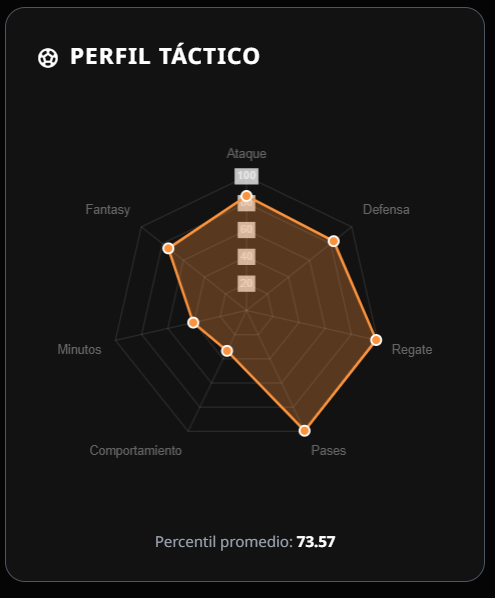
\includegraphics[width=0.3\textwidth]{./images/radar.png}
\caption{Radar chart de Pedri González.}
\end{figure}

Otro elemento especialmente relevante es la gestión de la plantilla mediante drag and drop. Esta funcionalidad aporta una interacción mucho más natural 
que la simple edición por formularios, ya que permite reorganizar jugadores visualmente dentro del campo. Además de mejorar la experiencia de uso, esta 
solución refuerza la comprensión táctica de la alineación y hace que el usuario perciba la gestión de su equipo como una acción directa e inmediata.

También merece mención el uso de explicaciones contextuales y percentiles en la ficha de jugador. La interfaz no se limita a mostrar estadísticas aisladas,
 sino que acompaña los datos con interpretaciones y comparativas que ayudan a entender el rendimiento del jugador dentro de su rol y de su contexto competitivo. 
 Esto convierte al frontend en una herramienta de análisis y apoyo a la decisión, no solo en un visor de datos.

\begin{figure}[h]
\centering
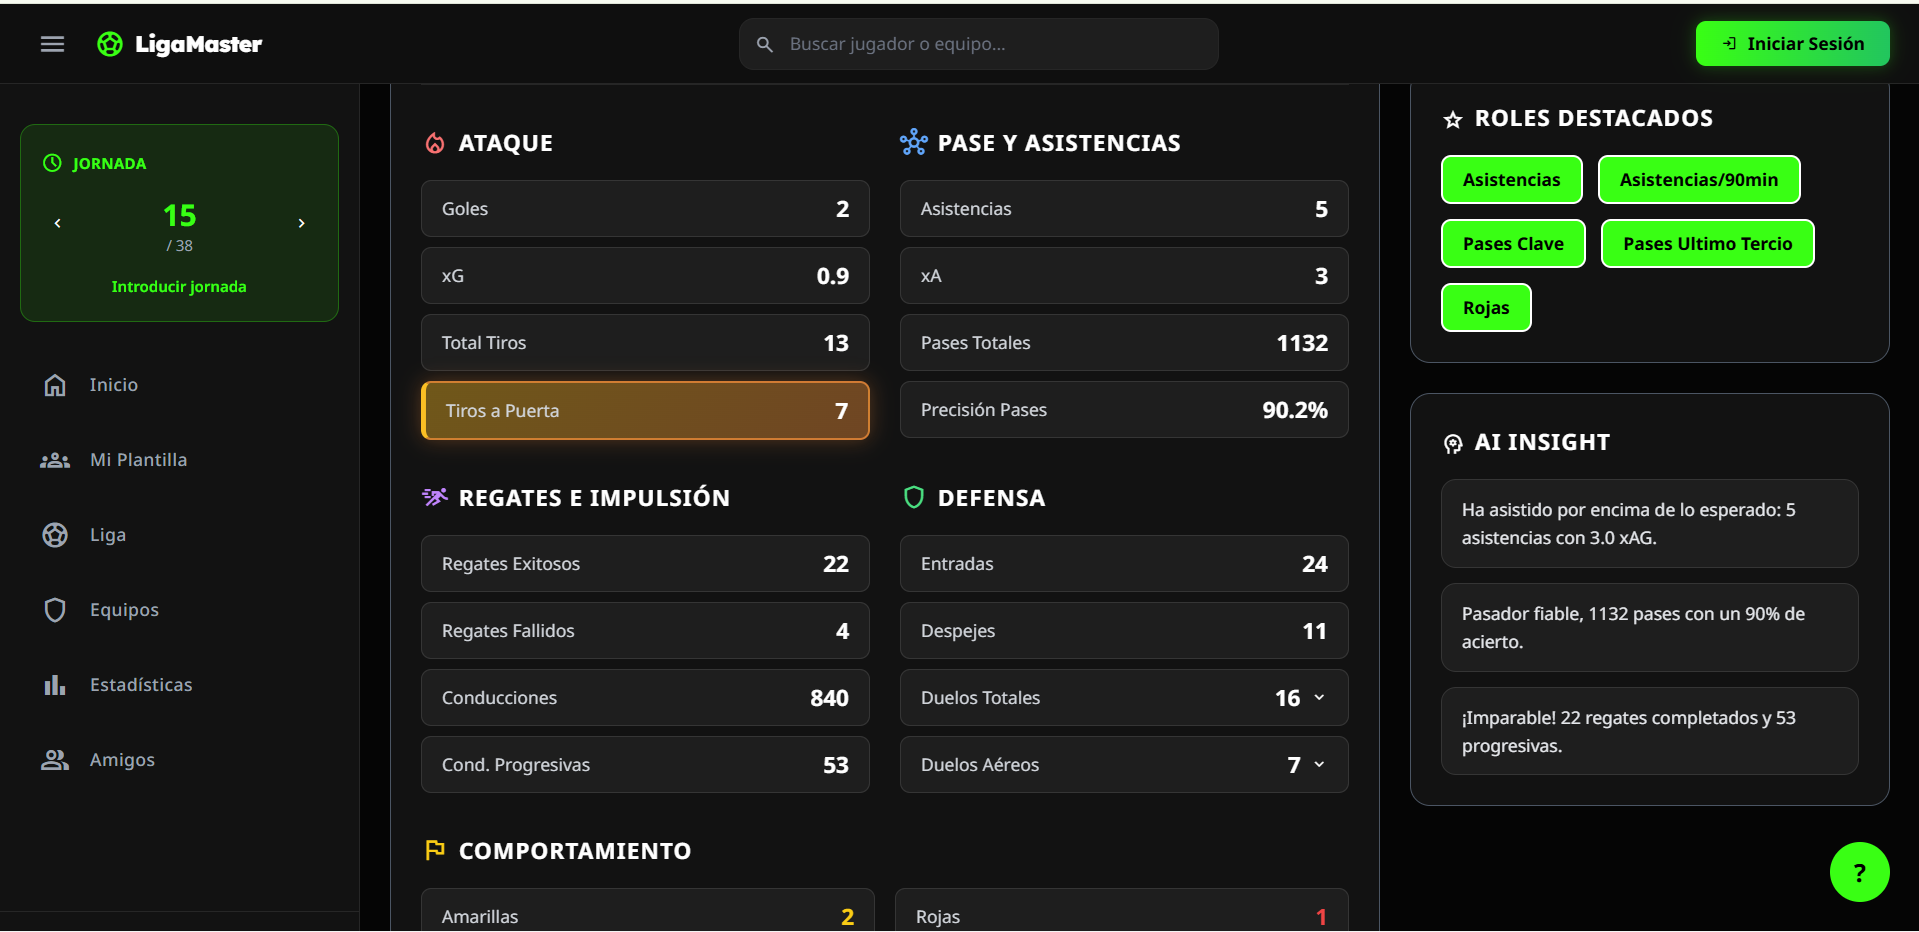
\includegraphics[width=0.8\textwidth]{./images/jugadorView.png}
\caption{Uso de percentiles y roles en la interfaz en la ficha de Pedri González.}
\end{figure}

Finalmente, se incorporó un tour guiado para facilitar la exploración inicial de la aplicación. Esta funcionalidad resulta útil porque introduce al usuario 
en las pantallas más importantes y reduce la curva de aprendizaje, especialmente en un sistema con varias capas de información y navegación.


\subsection{8.8 Principales problemas enfrentados}

A lo largo del ciclo de vida del proyecto, surgieron diversos obstáculos técnicos y metodológicos que obligaron a replantear decisiones de diseño y a aplicar soluciones
 creativas. Estos retos, lejos de ser simples contratiempos, permitieron profundizar en el conocimiento de las herramientas y en la robustez de la arquitectura final.

\subsubsection{8.8.1 Optimización del despliegue}
Durante las fases iniciales de desarrollo, se detectó un problema crítico de eficiencia en el flujo de trabajo con Docker. En las primeras versiones de la orquestación,
 cada vez que se levantaban los contenedores, el sistema procedía a borrar y recrear la base de datos desde cero por defecto.

Dada la magnitud del dataset y la complejidad del pipeline de scraping (que, como se ha detallado en el punto 8.2, incluye miles de registros estadísticos), este proceso de 
población inicial demoraba más de 20 minutos en cada arranque. Esta carga inicial bloqueante penalizaba severamente la productividad y la disponibilidad del servicio.

\textbf{Solución:} Se implementó una lógica de integridad en el componente \texttt{apps.py} (explicada en el punto 8.4). El sistema ahora realiza una auditoría de persistencia 
mediante consultas de salud (health checks) y comprobaciones de volumen. Si el sistema detecta que la base de datos ya está poblada, omite el flujo de carga masiva, reduciendo el 
tiempo de preparación de minutos a escasos segundos.

\subsubsection{8.8.2 Ambigüedad en el matching de entidades y barreras de scraping}
El proceso de unificar datos procedentes de tres fuentes heterogéneas (FBRef, FutbolFantasy y Transfermarkt) supuso un reto de limpieza de datos superior al previsto. La principal 
dificultad residió en la inconsistencia de los nombres de los futbolistas.

Casos como los de los hermanos Williams (Iñaki y Nico, I. Williams y N. Williams) en el Athletic Club, o jugadores con nombres extremadamente comunes como Eric García y Joan García, generaban colisiones en los algoritmos de búsqueda. 
A esto se sumó la política restrictiva de bloqueos por IP de los portales de origen, que identificaban las ráfagas de peticiones como tráfico malicioso.

\textbf{Solución:} Se abandonó la comparación simple por cadenas de texto en favor de la lógica difusa y el matching por contexto de partido (detallado en el punto 8.3). Además, para evadir los bloqueos, se diseñó 
la estrategia de backoff exponencial y la gestión de descargas locales controladas para los datos históricos más pesados.

\subsubsection{8.8.3 Refactorización arquitectónica: de Django Templates a React}
Originalmente, el frontend se concibió utilizando el sistema de vistas y plantillas nativo de Django. Sin embargo, a medida que los requisitos de interactividad crecieron (especialmente con el sistema de drag and drop
 y los gráficos en tiempo real), se hizo evidente que una arquitectura monolítica no era suficiente.

Se decidió migrar toda la capa de presentación a React. En un intento inicial por optimizar tiempos, se recurrió a herramientas de inteligencia artificial para automatizar la conversión de código Python/HTML a
 componentes JavaScript. No obstante, el resultado fue insatisfactorio: el código generado presentaba una deuda técnica inasumible, con errores de lógica en el manejo de hooks y una integración deficiente con la API.

\textbf{Lección aprendida:} La migración tuvo que realizarse de forma manual e íntegra. Aunque esto supuso una inversión de tiempo considerable y un retraso en el cronograma original, garantizó la calidad del código, 
la correcta gestión del estado global (como se analiza en el punto 8.7) y una experiencia de usuario fluida que la automatización no pudo alcanzar.

\subsubsection{8.8.4 Integridad predictiva: detección y corrección de Data Leakage}
Uno de los errores más sutiles pero peligrosos ocurrió durante el entrenamiento inicial de los modelos de Machine Learning. En las primeras aproximaciones, al no haber trabajado previamente con series temporales deportivas de esta escala, 
se aplicaron divisiones aleatorias de datos (random splits).

Esto provocó un fenómeno de data leakages: el modelo "predecía" el pasado utilizando información del futuro, arrojando métricas de precisión extraordinariamente altas que no se correspondían con la realidad. Al intentar
 predecir jornadas nuevas sin datos almacenados, el rendimiento caía drásticamente.

\textbf{Solución:} Se rediseñó por completo el motor de entrenamiento en el \texttt{BaseTrainer} (ver punto 8.4.2), imponiendo un corte temporal estricto. Se aseguró que para predecir la jornada $n$, el modelo solo tuviera acceso a datos
 de la jornada $n-1$ hacia atrás, garantizando así la validez científica de las predicciones y la utilidad real de la herramienta para el usuario.

La implementación del sistema ha sido un proceso iterativo de refinamiento técnico. La transición de un modelo monolítico a uno desacoplado, la superación de las barreras de extracción de datos y la corrección de sesgos en los modelos
 predictivos han consolidado una plataforma que no solo es funcional, sino también escalable y robusta ante las inconsistencias del mundo real. Los problemas enfrentados han servido para validar la arquitectura propuesta, demostrando que la integración de Machine Learning en entornos de producción exige un control riguroso tanto de la infraestructura como de la integridad de los datos.

\subsubsection{8.8.5 Elección del motor de búsqueda}

Durante el desarrollo del sistema, la elección del motor de búsqueda ha sido un aspecto clave debido a la necesidad de realizar consultas eficientes sobre grandes volúmenes de datos deportivos.

En una primera fase, se optó por utilizar \textbf{ElasticSearch}, aprovechando su integración con servicios gestionados en la nube y su potente sistema de indexación. Sin embargo, esta solución presentaba una limitación importante: tras un periodo inicial gratuito, el servicio requería una suscripción de pago, lo cual no se ajustaba a los requisitos del proyecto.

Como alternativa, se evaluó \textbf{OpenSearch}, un fork open-source de ElasticSearch que eliminaba dicha restricción económica. No obstante, durante las pruebas de despliegue se observó que su consumo de recursos era elevado, especialmente en términos de memoria RAM. Esto lo hacía inviable en entornos con recursos limitados, como las máquinas virtuales gratuitas o de bajo coste disponibles en Azure.

\textbf{Solución:} Finalmente, se optó por \textbf{MeiliSearch}, un motor de búsqueda ligero y optimizado para rendimiento, que permite su despliegue en entornos con recursos reducidos sin comprometer significativamente la velocidad de respuesta. Esta elección permitió mantener la funcionalidad de búsqueda avanzada dentro de las restricciones de infraestructura del proyecto, asegurando al mismo tiempo una experiencia de usuario fluida.

Esta transición evidencia la importancia de considerar no solo las capacidades técnicas de una herramienta, sino también su viabilidad en entornos reales de despliegue, especialmente cuando existen limitaciones económicas y de recursos.
\subsubsection{8.8.6 Despliegue en producción}

El despliegue en producción planteó desafíos significativos, especialmente en relación con la gestión de costes y la sostenibilidad de la infraestructura a lo largo del tiempo.

Inicialmente, se consideró una arquitectura monolítica basada en una única máquina virtual en Azure que albergara todos los componentes del sistema. Sin embargo, durante la fase de estimación de costes se determinó que esta solución supondría un gasto mensual mayor al crédito estundiantil de Azure, lo cual resultaba inviable para un proyecto académico cuyo objetivo es mantenerse accesible durante varios meses para su evaluación.

\textbf{Solución:} Se rediseñó la arquitectura hacia un modelo distribuido, delegando distintos componentes en servicios especializados y, en muchos casos, con planes gratuitos o de bajo coste:
\begin{itemize}
    \item El \textbf{frontend} se desplegó en Vercel, aprovechando su integración con aplicaciones SPA y su red de distribución global.
    \item La \textbf{base de datos} se externalizó a Supabase, proporcionando un servicio PostgreSQL gestionado.
    \item El sistema de \textbf{caché} se implementó mediante Upstash Redis, optimizado para entornos serverless.
    \item En Azure se mantuvieron únicamente los componentes críticos: el \textbf{backend en Django} y el motor de búsqueda \textbf{MeiliSearch}.
\end{itemize}

Esta estrategia permitió reducir drásticamente los costes de infraestructura, manteniendo al mismo tiempo la escalabilidad y disponibilidad del sistema. Además, el enfoque distribuido mejora la resiliencia de la aplicación y refleja una arquitectura más cercana a entornos reales de producción.

En conclusión, el proceso de despliegue no solo ha servido para optimizar recursos, sino también para validar decisiones arquitectónicas orientadas a la sostenibilidad y eficiencia del sistema.